% Options for packages loaded elsewhere
\PassOptionsToPackage{unicode}{hyperref}
\PassOptionsToPackage{hyphens}{url}
%
\documentclass[
]{article}
\title{Getting the most out of surveys: Multilevel Regression And
Poststratification}
\author{Joseph T. Ornstein\footnote{Department of Political Science,
  University of Georgia}}
\date{}

\usepackage{amsmath,amssymb}
\usepackage{lmodern}
\usepackage{iftex}
\ifPDFTeX
  \usepackage[T1]{fontenc}
  \usepackage[utf8]{inputenc}
  \usepackage{textcomp} % provide euro and other symbols
\else % if luatex or xetex
  \usepackage{unicode-math}
  \defaultfontfeatures{Scale=MatchLowercase}
  \defaultfontfeatures[\rmfamily]{Ligatures=TeX,Scale=1}
\fi
% Use upquote if available, for straight quotes in verbatim environments
\IfFileExists{upquote.sty}{\usepackage{upquote}}{}
\IfFileExists{microtype.sty}{% use microtype if available
  \usepackage[]{microtype}
  \UseMicrotypeSet[protrusion]{basicmath} % disable protrusion for tt fonts
}{}
\makeatletter
\@ifundefined{KOMAClassName}{% if non-KOMA class
  \IfFileExists{parskip.sty}{%
    \usepackage{parskip}
  }{% else
    \setlength{\parindent}{0pt}
    \setlength{\parskip}{6pt plus 2pt minus 1pt}}
}{% if KOMA class
  \KOMAoptions{parskip=half}}
\makeatother
\usepackage{xcolor}
\IfFileExists{xurl.sty}{\usepackage{xurl}}{} % add URL line breaks if available
\IfFileExists{bookmark.sty}{\usepackage{bookmark}}{\usepackage{hyperref}}
\hypersetup{
  pdftitle={Getting the most out of surveys: Multilevel Regression And Poststratification},
  pdfauthor={Joseph T. Ornstein},
  pdfkeywords={survey weighting, small area estimation, public opinion,
R programming, monte carlo simulation},
  hidelinks,
  pdfcreator={LaTeX via pandoc}}
\urlstyle{same} % disable monospaced font for URLs
\usepackage[margin=1in]{geometry}
\usepackage{color}
\usepackage{fancyvrb}
\newcommand{\VerbBar}{|}
\newcommand{\VERB}{\Verb[commandchars=\\\{\}]}
\DefineVerbatimEnvironment{Highlighting}{Verbatim}{commandchars=\\\{\}}
% Add ',fontsize=\small' for more characters per line
\usepackage{framed}
\definecolor{shadecolor}{RGB}{248,248,248}
\newenvironment{Shaded}{\begin{snugshade}}{\end{snugshade}}
\newcommand{\AlertTok}[1]{\textcolor[rgb]{0.94,0.16,0.16}{#1}}
\newcommand{\AnnotationTok}[1]{\textcolor[rgb]{0.56,0.35,0.01}{\textbf{\textit{#1}}}}
\newcommand{\AttributeTok}[1]{\textcolor[rgb]{0.77,0.63,0.00}{#1}}
\newcommand{\BaseNTok}[1]{\textcolor[rgb]{0.00,0.00,0.81}{#1}}
\newcommand{\BuiltInTok}[1]{#1}
\newcommand{\CharTok}[1]{\textcolor[rgb]{0.31,0.60,0.02}{#1}}
\newcommand{\CommentTok}[1]{\textcolor[rgb]{0.56,0.35,0.01}{\textit{#1}}}
\newcommand{\CommentVarTok}[1]{\textcolor[rgb]{0.56,0.35,0.01}{\textbf{\textit{#1}}}}
\newcommand{\ConstantTok}[1]{\textcolor[rgb]{0.00,0.00,0.00}{#1}}
\newcommand{\ControlFlowTok}[1]{\textcolor[rgb]{0.13,0.29,0.53}{\textbf{#1}}}
\newcommand{\DataTypeTok}[1]{\textcolor[rgb]{0.13,0.29,0.53}{#1}}
\newcommand{\DecValTok}[1]{\textcolor[rgb]{0.00,0.00,0.81}{#1}}
\newcommand{\DocumentationTok}[1]{\textcolor[rgb]{0.56,0.35,0.01}{\textbf{\textit{#1}}}}
\newcommand{\ErrorTok}[1]{\textcolor[rgb]{0.64,0.00,0.00}{\textbf{#1}}}
\newcommand{\ExtensionTok}[1]{#1}
\newcommand{\FloatTok}[1]{\textcolor[rgb]{0.00,0.00,0.81}{#1}}
\newcommand{\FunctionTok}[1]{\textcolor[rgb]{0.00,0.00,0.00}{#1}}
\newcommand{\ImportTok}[1]{#1}
\newcommand{\InformationTok}[1]{\textcolor[rgb]{0.56,0.35,0.01}{\textbf{\textit{#1}}}}
\newcommand{\KeywordTok}[1]{\textcolor[rgb]{0.13,0.29,0.53}{\textbf{#1}}}
\newcommand{\NormalTok}[1]{#1}
\newcommand{\OperatorTok}[1]{\textcolor[rgb]{0.81,0.36,0.00}{\textbf{#1}}}
\newcommand{\OtherTok}[1]{\textcolor[rgb]{0.56,0.35,0.01}{#1}}
\newcommand{\PreprocessorTok}[1]{\textcolor[rgb]{0.56,0.35,0.01}{\textit{#1}}}
\newcommand{\RegionMarkerTok}[1]{#1}
\newcommand{\SpecialCharTok}[1]{\textcolor[rgb]{0.00,0.00,0.00}{#1}}
\newcommand{\SpecialStringTok}[1]{\textcolor[rgb]{0.31,0.60,0.02}{#1}}
\newcommand{\StringTok}[1]{\textcolor[rgb]{0.31,0.60,0.02}{#1}}
\newcommand{\VariableTok}[1]{\textcolor[rgb]{0.00,0.00,0.00}{#1}}
\newcommand{\VerbatimStringTok}[1]{\textcolor[rgb]{0.31,0.60,0.02}{#1}}
\newcommand{\WarningTok}[1]{\textcolor[rgb]{0.56,0.35,0.01}{\textbf{\textit{#1}}}}
\usepackage{graphicx}
\makeatletter
\def\maxwidth{\ifdim\Gin@nat@width>\linewidth\linewidth\else\Gin@nat@width\fi}
\def\maxheight{\ifdim\Gin@nat@height>\textheight\textheight\else\Gin@nat@height\fi}
\makeatother
% Scale images if necessary, so that they will not overflow the page
% margins by default, and it is still possible to overwrite the defaults
% using explicit options in \includegraphics[width, height, ...]{}
\setkeys{Gin}{width=\maxwidth,height=\maxheight,keepaspectratio}
% Set default figure placement to htbp
\makeatletter
\def\fps@figure{htbp}
\makeatother
\setlength{\emergencystretch}{3em} % prevent overfull lines
\providecommand{\tightlist}{%
  \setlength{\itemsep}{0pt}\setlength{\parskip}{0pt}}
\setcounter{secnumdepth}{5}
\newlength{\cslhangindent}
\setlength{\cslhangindent}{1.5em}
\newlength{\csllabelwidth}
\setlength{\csllabelwidth}{3em}
\newlength{\cslentryspacingunit} % times entry-spacing
\setlength{\cslentryspacingunit}{\parskip}
\newenvironment{CSLReferences}[2] % #1 hanging-ident, #2 entry spacing
 {% don't indent paragraphs
  \setlength{\parindent}{0pt}
  % turn on hanging indent if param 1 is 1
  \ifodd #1
  \let\oldpar\par
  \def\par{\hangindent=\cslhangindent\oldpar}
  \fi
  % set entry spacing
  \setlength{\parskip}{#2\cslentryspacingunit}
 }%
 {}
\usepackage{calc}
\newcommand{\CSLBlock}[1]{#1\hfill\break}
\newcommand{\CSLLeftMargin}[1]{\parbox[t]{\csllabelwidth}{#1}}
\newcommand{\CSLRightInline}[1]{\parbox[t]{\linewidth - \csllabelwidth}{#1}\break}
\newcommand{\CSLIndent}[1]{\hspace{\cslhangindent}#1}
\ifLuaTeX
  \usepackage{selnolig}  % disable illegal ligatures
\fi

\begin{document}
\maketitle
\begin{abstract}
Good causal inference requires good measurement; even the most
thoughtfully designed research can be derailed by noisy data. Because
policy scholars are often interested in public opinion as a key
dependent or independent variable, paying careful attention to the
sources of measurement error from surveys is an essential step for
detecting causation. This chapter introduces multilevel regression and
poststratification (MRP), an approach to adjusting public opinion
estimates to account for observed imbalances between the survey sample
and population of interest. It covers the history of MRP, recent
advances, a running example with code, and concludes with a discussion
of best practices and limitations of the approach.
\end{abstract}

\hypertarget{learning-objectives}{%
\section{Learning Objectives}\label{learning-objectives}}

By the end of this chapter, you will be able to:

\begin{itemize}
\item
  Explain the motivation for MRP and the circumstances under which it is
  appropriate to implement.
\item
  Describe the two steps in producing MRP estimates: model fitting and
  postsratification.
\item
  Generate MRP estimates by adapting the provided sample code.
\item
  Implement more sophisticated variants of MRP, including stacked
  regression and postratification (SRP) or multilevel regression and
  synthetic poststratification (MrsP) where appropriate.
\end{itemize}

\hypertarget{introduction}{%
\section{Introduction}\label{introduction}}

Often researchers would like to measure public opinion on some policy
issue, but the surveys we use to do so are unrepresentative in some
important way. Perhaps their respondents come from a convenience sample
(Wang et al. 2015), or non-response bias skews an otherwise random
sample. Or perhaps the data is representative of some larger population
(i.e.~a country-level random sample), but contains too few observations
to make inferences about a subgroup of interest. Even the largest US
public opinion surveys do not have enough respondents to make reliable
inferences about lower-level political entities like states or
municipalities. Conclusions drawn from low frequency observations --
even in a large sample survey -- can be wildly misleading (Ansolabehere,
Luks, and Schaffner 2015).

This presents a challenge for public opinion research: how to take
unrepresentative survey data and adjust it so that it is useful for our
particular research question. In this chapter, I will demonstrate a
method called \textbf{multilevel regression and poststratification}
(MRP). Using this approach, the researcher first constructs a model of
public opinion (multilevel regression) and then reweights the model's
predictions based on the observed characteristics of the population of
interest (poststratification). In the sections to follow, I will
describe this approach in detail, and will accompany this explanation
with replication code in the \texttt{R} statistical language.

MRP was first introduced by Gelman and Little (1997), and in the
subsequent decades it has helped address a diverse set of research
questions in political science. These range from generating election
forecasts using unrepresentative survey data (Wang et al. 2015) to
assessing the responsiveness of state (Lax and Phillips 2012) and local
policymakers (Tausanovitch and Warshaw 2014) to their constituents'
policy preferences.

In the following sections, I will illustrate how MRP can improve
estimates of small area public opinion. Our running example will be
drawn from the Cooperative Election Study (Schaffner, Ansolabehere, and
Luks 2021), a 50,000+ respondent study of voters in the United States.
The 2020 wave of the study includes a question asking respondents
whether they support a policy that would ``decrease the number of police
on the street by 10 percent, and increase funding for other public
services.'' Since police reform is a policy issue on which US local
governments have a significant amount of autonomy, it would be useful to
know how opinions on this issue vary from place to place without having
to conduct separate, costly surveys in each area.

As we will see, the accuracy of our MRP estimates depends critically on
whether the first-stage model makes good out-of-sample predictions. The
best first-stage models are \emph{regularized} (Gelman 2018) to avoid
both over- and under-fitting to the survey data. Regularized ensemble
models (Ornstein 2020) with group-level predictors tend to produce the
best estimates, especially when trained on large datasets.

\hypertarget{how-it-works}{%
\section{How It Works}\label{how-it-works}}

Perhaps the core insight motivating MRP is that unrepresentative surveys
can be , while a survey sample may be unrepresentative

TODO:

\begin{itemize}
\tightlist
\item
  A non-technical ``narrative'' section, which links the chapter to the
  goal of detecting causation in the social sciences. Good measurement
  is as central to causal inference as a good research design, both for
  reasons of precision (better measurement implies less noisy
  estimands), and external validity. So much of the data we use for
  causal inference in the social sciences comes from surveys. Worried
  about whether the survey is representative of the population you're
  interested in, or perhaps you're interested in a subpopulation or
  small area and you don't have a representative survey data for that
  group. MRP helps by making use of all the information available in a
  survey, making inferences about individuals \emph{not} in the survey
  based on the characteristics of individuals \emph{in} the survey.
\end{itemize}

\hypertarget{running-example}{%
\section{Running Example}\label{running-example}}

To demonstrate how MRP works, we'll consider an example where we know
the true population-level estimands, and can explore how various
refinements to the method can improve predictive accuracy. This approach
mirrors Buttice and Highton (2013), who use disaggregated ressponses
from large-scale US survey of voters as the target. The Cooperative
Election Study data is available
\href{https://dataverse.harvard.edu/dataset.xhtml?persistentId=doi\%3A10.7910/DVN/E9N6PH}{here},
and we'll be using a tidied version of the dataset created by the
\texttt{R/cleanup-ces-2020.R} script.\footnote{All replication code and
  data will be made available on a public repository. Throughout, I will
  use R functions from the ``tidyverse'' to make the code more
  human-readable.}

\begin{Shaded}
\begin{Highlighting}[]
\FunctionTok{library}\NormalTok{(tidyverse)}
\FunctionTok{library}\NormalTok{(ggrepel)}

\FunctionTok{load}\NormalTok{(}\StringTok{\textquotesingle{}data/CES{-}2020.RData\textquotesingle{}}\NormalTok{)}
\end{Highlighting}
\end{Shaded}

This tidied version of the data only includes the 33 states with at
least 500 respondents. First, let's plot the percent of CES respondents
who supported ``defunding'' the police\footnote{Obviously that phrase
  means different things to different people. In this case, we'll stick
  with the CES proposed policy of reducing police staffing by 10\% and
  diverting those expenditures to other priorities.} by state.

\begin{Shaded}
\begin{Highlighting}[]
\NormalTok{truth }\OtherTok{\textless{}{-}}\NormalTok{ ces }\SpecialCharTok{\%\textgreater{}\%} 
  \FunctionTok{group\_by}\NormalTok{(abb) }\SpecialCharTok{\%\textgreater{}\%} 
  \FunctionTok{summarize}\NormalTok{(}\AttributeTok{truth =} \FunctionTok{mean}\NormalTok{(defund\_police))}

\NormalTok{truth }\SpecialCharTok{\%\textgreater{}\%} 
  \FunctionTok{mutate}\NormalTok{(}\AttributeTok{abb =} \FunctionTok{fct\_reorder}\NormalTok{(abb, truth)) }\SpecialCharTok{\%\textgreater{}\%} 
  \FunctionTok{ggplot}\NormalTok{(}\AttributeTok{mapping =} \FunctionTok{aes}\NormalTok{(}\AttributeTok{x=}\NormalTok{truth, }\AttributeTok{y=}\NormalTok{abb)) }\SpecialCharTok{+}
  \FunctionTok{geom\_point}\NormalTok{(}\AttributeTok{alpha =} \FloatTok{0.7}\NormalTok{) }\SpecialCharTok{+}
  \FunctionTok{labs}\NormalTok{(}\AttributeTok{x =} \StringTok{\textquotesingle{}Percent Who Support Police Reform Policy\textquotesingle{}}\NormalTok{,}
       \AttributeTok{y =} \StringTok{\textquotesingle{}State\textquotesingle{}}\NormalTok{) }\SpecialCharTok{+}
  \FunctionTok{theme\_minimal}\NormalTok{()}
\end{Highlighting}
\end{Shaded}

\begin{figure}
\centering
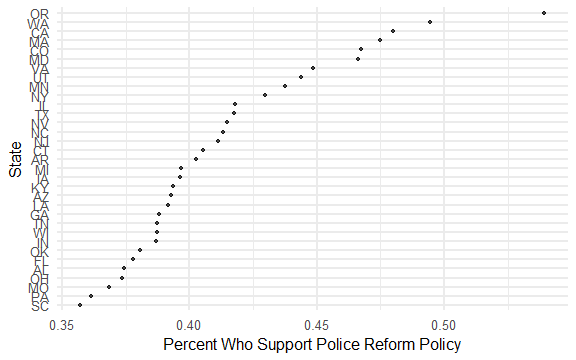
\includegraphics{chapter_files/figure-latex/truth-1.pdf}
\caption{The percent of CES respondents in each state who support
reducing police budgets. These are our target estimands.}
\end{figure}

Oregon is the only state where a majority of respondents supported this
policy proposal. And note that Figure 1 likely \emph{overstates} the
percent of the total population that support such a policy, since
self-identified Democrats are over-represented in the CES sample. But
nevertheless, these population-level parameters will be a useful target
to estimate with MRP.

\hypertarget{draw-a-sample}{%
\subsection{Draw a Sample}\label{draw-a-sample}}

Suppose that we did not have access to the entire CES dataset, but only
to a random sample of 1,000 respondents. How good of a job can we do at
estimating those state-level means?

\begin{Shaded}
\begin{Highlighting}[]
\NormalTok{sample\_data }\OtherTok{\textless{}{-}}\NormalTok{ ces }\SpecialCharTok{\%\textgreater{}\%} 
  \FunctionTok{slice\_sample}\NormalTok{(}\AttributeTok{n =} \DecValTok{1000}\NormalTok{)}
\end{Highlighting}
\end{Shaded}

\begin{Shaded}
\begin{Highlighting}[]
\NormalTok{sample\_summary }\OtherTok{\textless{}{-}}\NormalTok{ sample\_data }\SpecialCharTok{\%\textgreater{}\%} 
  \FunctionTok{group\_by}\NormalTok{(abb) }\SpecialCharTok{\%\textgreater{}\%} 
  \FunctionTok{summarize}\NormalTok{(}\AttributeTok{estimate =} \FunctionTok{mean}\NormalTok{(defund\_police),}
            \AttributeTok{num =} \FunctionTok{n}\NormalTok{())}

\NormalTok{sample\_summary}
\end{Highlighting}
\end{Shaded}

\begin{verbatim}
## # A tibble: 33 x 3
##    abb   estimate   num
##    <chr>    <dbl> <int>
##  1 AL       0.55     20
##  2 AR       0         4
##  3 AZ       0.438    16
##  4 CA       0.435    85
##  5 CO       0.478    23
##  6 CT       0.375     8
##  7 FL       0.402    87
##  8 GA       0.346    26
##  9 IA       0.308    13
## 10 IL       0.28     50
## # ... with 23 more rows
\end{verbatim}

In a sample with only 1,000 respondents, there are several states with
very few (or no) respondents. Notice, for example, that this sample
includes only four respondents from Arkansas, of whom zero support
reducing police budgets. Simply disaggregating and taking sample means
is unlikely to yield good estimates, as you can see by comparing those
sample means against the truth.

\begin{Shaded}
\begin{Highlighting}[]
\CommentTok{\# a function to plot the state{-}level estimates against the truth}
\NormalTok{compare\_to\_truth }\OtherTok{\textless{}{-}} \ControlFlowTok{function}\NormalTok{(estimates, truth)\{}
  
\NormalTok{  d }\OtherTok{\textless{}{-}} \FunctionTok{left\_join}\NormalTok{(estimates, truth, }\AttributeTok{by =} \StringTok{\textquotesingle{}abb\textquotesingle{}}\NormalTok{)}
  
  \FunctionTok{ggplot}\NormalTok{(}\AttributeTok{data =}\NormalTok{ d,}
         \AttributeTok{mapping =} \FunctionTok{aes}\NormalTok{(}\AttributeTok{x=}\NormalTok{estimate,}
                       \AttributeTok{y=}\NormalTok{truth,}
                       \AttributeTok{label=}\NormalTok{abb)) }\SpecialCharTok{+}
  \FunctionTok{geom\_point}\NormalTok{(}\AttributeTok{alpha =} \FloatTok{0.5}\NormalTok{) }\SpecialCharTok{+}
  \FunctionTok{geom\_text\_repel}\NormalTok{() }\SpecialCharTok{+}
  \FunctionTok{theme\_minimal}\NormalTok{() }\SpecialCharTok{+}
  \FunctionTok{geom\_abline}\NormalTok{(}\AttributeTok{intercept =} \DecValTok{0}\NormalTok{, }\AttributeTok{slope =} \DecValTok{1}\NormalTok{, }\AttributeTok{linetype =} \StringTok{\textquotesingle{}dashed\textquotesingle{}}\NormalTok{) }\SpecialCharTok{+}
  \FunctionTok{labs}\NormalTok{(}\AttributeTok{x =} \StringTok{\textquotesingle{}Estimate\textquotesingle{}}\NormalTok{,}
       \AttributeTok{y =} \StringTok{\textquotesingle{}Truth\textquotesingle{}}\NormalTok{,}
       \AttributeTok{caption =} \FunctionTok{paste0}\NormalTok{(}\StringTok{\textquotesingle{}Correlation = \textquotesingle{}}\NormalTok{, }\FunctionTok{round}\NormalTok{(}\FunctionTok{cor}\NormalTok{(d}\SpecialCharTok{$}\NormalTok{estimate, d}\SpecialCharTok{$}\NormalTok{truth), }\DecValTok{2}\NormalTok{), }
                        \StringTok{\textquotesingle{}, Mean Absolute Error = \textquotesingle{}}\NormalTok{, }\FunctionTok{round}\NormalTok{(}\FunctionTok{mean}\NormalTok{(}\FunctionTok{abs}\NormalTok{(d}\SpecialCharTok{$}\NormalTok{estimate }\SpecialCharTok{{-}}\NormalTok{ d}\SpecialCharTok{$}\NormalTok{truth)), }\DecValTok{3}\NormalTok{)))}
\NormalTok{\}}

\FunctionTok{compare\_to\_truth}\NormalTok{(sample\_summary, truth)}
\end{Highlighting}
\end{Shaded}

\begin{figure}
\centering
\includegraphics{chapter_files/figure-latex/compare-disaggregation-1.pdf}
\caption{Esimates from disaggregated sample data}
\end{figure}

These are clearly poor estimates of state-level public opinion. The four
respondents from Arksansas simply do not give us enough information to
adequately measure public opinion in that state. But one of the key
insights behind MRP is that the respondents from Arkansas are not the
only respondents who can give us information about Arkansas! There are
other respondents in, for example, Missouri, that are similar to
Arkansas residents on their observed characteristics. If we can
determine the characteristics that predict support for police reform
using the entire survey sample, then we can use those predictions --
combined with demographic information about Arkansans -- to generate
better estimates. The trick, in essence, is that our estimate for
Arkansas will be borrowing information from similar respondents in other
states.

The method proceeds in three steps.

\hypertarget{step-1-fit-a-model}{%
\subsection{Step 1: Fit a Model}\label{step-1-fit-a-model}}

First, we fit a model of our outcome, using observed characteristics of
the survey respondents as predictors. To demonstrate, let's fit a simple
logistic regression model including only four demographic predictors:
gender, education, race, and age.

\begin{Shaded}
\begin{Highlighting}[]
\NormalTok{model }\OtherTok{\textless{}{-}} \FunctionTok{glm}\NormalTok{(defund\_police }\SpecialCharTok{\textasciitilde{}}
\NormalTok{              gender }\SpecialCharTok{+}\NormalTok{ educ }\SpecialCharTok{+}\NormalTok{ race }\SpecialCharTok{+}\NormalTok{ age,}
            \AttributeTok{data =}\NormalTok{ sample\_data,}
            \AttributeTok{family =} \StringTok{\textquotesingle{}binomial\textquotesingle{}}\NormalTok{)}
\end{Highlighting}
\end{Shaded}

\hypertarget{step-2-construct-the-poststratification-frame}{%
\subsection{Step 2: Construct the Poststratification
Frame}\label{step-2-construct-the-poststratification-frame}}

The poststratification stage requires the researcher to know (or
estimate) the joint frequency distribution of predictor variables in
each state. This information is stored in a ``poststratification
frame,'' a matrix where each row is a unique combination of
characteristics, along with the observed frequency of that combination.
Often, one constructs this frequency distribution from Census micro-data
(Lax and Phillips 2009). For our demonstration, I will compute it
directly from the CES.

\begin{Shaded}
\begin{Highlighting}[]
\NormalTok{psframe }\OtherTok{\textless{}{-}}\NormalTok{ ces }\SpecialCharTok{\%\textgreater{}\%} 
  \FunctionTok{count}\NormalTok{(abb, gender, educ, race, age)}

\FunctionTok{head}\NormalTok{(psframe)}
\end{Highlighting}
\end{Shaded}

\begin{verbatim}
## # A tibble: 6 x 6
##   abb   gender educ   race    age     n
##   <chr> <chr>  <chr>  <chr> <dbl> <int>
## 1 AL    Female 2_year Black    26     1
## 2 AL    Female 2_year Black    27     2
## 3 AL    Female 2_year Black    29     1
## 4 AL    Female 2_year Black    31     1
## 5 AL    Female 2_year Black    34     2
## 6 AL    Female 2_year Black    35     2
\end{verbatim}

\hypertarget{step-3-predict-and-poststratify}{%
\subsection{Step 3: Predict and
Poststratify}\label{step-3-predict-and-poststratify}}

With the model and poststratification frame in hand, the final step is
to generate frequency-weighted predictions of public opinion. For each
cell in the poststratification frame, append the model's predicted
probability of supporting police defunding.

\begin{Shaded}
\begin{Highlighting}[]
\NormalTok{psframe}\SpecialCharTok{$}\NormalTok{predicted\_probability }\OtherTok{\textless{}{-}} \FunctionTok{predict}\NormalTok{(model, psframe, }\AttributeTok{type =} \StringTok{\textquotesingle{}response\textquotesingle{}}\NormalTok{)}
\end{Highlighting}
\end{Shaded}

Then the poststratified estimates are the frequency-weighted means of
those predictions.

\begin{Shaded}
\begin{Highlighting}[]
\NormalTok{poststratified\_estimates }\OtherTok{\textless{}{-}}\NormalTok{ psframe }\SpecialCharTok{\%\textgreater{}\%} 
  \FunctionTok{group\_by}\NormalTok{(abb) }\SpecialCharTok{\%\textgreater{}\%} 
  \FunctionTok{summarize}\NormalTok{(}\AttributeTok{estimate =} \FunctionTok{weighted.mean}\NormalTok{(predicted\_probability, n))}
\end{Highlighting}
\end{Shaded}

Let's see how these estimates compare with the known values (Figure 3).

\begin{Shaded}
\begin{Highlighting}[]
\FunctionTok{compare\_to\_truth}\NormalTok{(poststratified\_estimates, truth)}
\end{Highlighting}
\end{Shaded}

\begin{figure}
\centering
\includegraphics{chapter_files/figure-latex/compare-to-truth-1.pdf}
\caption{Underfit MRP estimates from complete pooling model}
\end{figure}

These estimates, though still imperfectly correlated with the truth, are
much better than the previous estimates from disaggregation. Notice, in
particular, that the estimate for Arkansas went from 0\% to roughly
39\%, reflecting the significant improvement that comes from using more
information than the four Arkansans in our sample can provide.

But we can still do better. In the following sections, I will show how
successive improvements to the first-stage model can yield more reliable
poststratified estimates.

\hypertarget{beware-overfitting}{%
\subsection{Beware Overfitting}\label{beware-overfitting}}

A common instinct among social scientists building models is to take a
``kitchen sink'' approach, including as many explanatory variables as
possible (Achen 2005). This is counterproductive when the objective is
out-of-sample predictive accuracy. To illustrate, let's estimate a model
with a separate intercept term for each state -- a ``fixed effects''
model. Because our sample contains several states with very few
observations, these state-specific intercepts will be over-fit to
sampling variability.

\begin{Shaded}
\begin{Highlighting}[]
\CommentTok{\# fit the model}
\NormalTok{model2 }\OtherTok{\textless{}{-}} \FunctionTok{glm}\NormalTok{(defund\_police }\SpecialCharTok{\textasciitilde{}}
\NormalTok{              gender }\SpecialCharTok{+}\NormalTok{ educ }\SpecialCharTok{+}\NormalTok{ race }\SpecialCharTok{+}\NormalTok{ age }\SpecialCharTok{+}
\NormalTok{                abb,}
            \AttributeTok{data =}\NormalTok{ sample\_data,}
            \AttributeTok{family =} \StringTok{\textquotesingle{}binomial\textquotesingle{}}\NormalTok{)}

\CommentTok{\# construct the poststratification frame}
\NormalTok{psframe }\OtherTok{\textless{}{-}}\NormalTok{ ces }\SpecialCharTok{\%\textgreater{}\%} 
  \FunctionTok{count}\NormalTok{(abb, gender, educ, race, age)}

\CommentTok{\# make predictions}
\NormalTok{psframe}\SpecialCharTok{$}\NormalTok{predicted\_probability }\OtherTok{\textless{}{-}} \FunctionTok{predict}\NormalTok{(model2, psframe, }\AttributeTok{type =} \StringTok{\textquotesingle{}response\textquotesingle{}}\NormalTok{)}

\CommentTok{\# poststratify}
\NormalTok{poststratified\_estimates }\OtherTok{\textless{}{-}}\NormalTok{ psframe }\SpecialCharTok{\%\textgreater{}\%} 
  \FunctionTok{group\_by}\NormalTok{(abb) }\SpecialCharTok{\%\textgreater{}\%} 
  \FunctionTok{summarize}\NormalTok{(}\AttributeTok{estimate =} \FunctionTok{weighted.mean}\NormalTok{(predicted\_probability, n))}


\FunctionTok{compare\_to\_truth}\NormalTok{(poststratified\_estimates, truth)}
\end{Highlighting}
\end{Shaded}

\begin{figure}
\centering
\includegraphics{chapter_files/figure-latex/unnamed-chunk-1-1.pdf}
\caption{Overfit MRP estimates from fixed effects model}
\end{figure}

These poststratified estimates perform about as well as the
disaggregated estimates from Figure 2. Because each state's intercept is
estimated separately, the over-fit model foregoes the advantages of
``partial pooling'' (Park, Gelman, and Bafumi 2004), borrowing
information from respondents in other states. Note that the estimate for
Arkansas is once again 0\%.

\hypertarget{partial-pooling}{%
\subsection{Partial Pooling}\label{partial-pooling}}

A better approach is to estimate a multilevel model (alternatively known
as ``varying-intercepts'' or ``random effects'' model), including
group-level covariates. In the model below, I estimate varying
intercepts by US Census division, including the state's 2020 Democratic
vote share as a covariate. The result is a marked improvement over
Figure 3 (particularly for west coast states like Oregon, Washington,
and California).

\begin{Shaded}
\begin{Highlighting}[]
\FunctionTok{library}\NormalTok{(lme4)}

\CommentTok{\# fit the model}
\NormalTok{model3 }\OtherTok{\textless{}{-}} \FunctionTok{glmer}\NormalTok{(defund\_police }\SpecialCharTok{\textasciitilde{}}\NormalTok{  gender }\SpecialCharTok{+}\NormalTok{ educ }\SpecialCharTok{+}\NormalTok{ race }\SpecialCharTok{+}\NormalTok{ age }\SpecialCharTok{+}
\NormalTok{                (}\DecValTok{1} \SpecialCharTok{+}\NormalTok{ biden\_vote\_share }\SpecialCharTok{|}\NormalTok{ division), }
                 \AttributeTok{data =}\NormalTok{ sample\_data,}
                 \AttributeTok{family =} \StringTok{\textquotesingle{}binomial\textquotesingle{}}\NormalTok{)}

\CommentTok{\# construct the poststratification frame}
\NormalTok{psframe }\OtherTok{\textless{}{-}}\NormalTok{ ces }\SpecialCharTok{\%\textgreater{}\%} 
  \FunctionTok{count}\NormalTok{(abb, gender, educ, race, age, division, biden\_vote\_share)}

\CommentTok{\# make predictions}
\NormalTok{psframe}\SpecialCharTok{$}\NormalTok{predicted\_probability }\OtherTok{\textless{}{-}} \FunctionTok{predict}\NormalTok{(model3, psframe, }\AttributeTok{type =} \StringTok{\textquotesingle{}response\textquotesingle{}}\NormalTok{)}

\CommentTok{\# poststratify}
\NormalTok{poststratified\_estimates }\OtherTok{\textless{}{-}}\NormalTok{ psframe }\SpecialCharTok{\%\textgreater{}\%} 
  \FunctionTok{group\_by}\NormalTok{(abb) }\SpecialCharTok{\%\textgreater{}\%} 
  \FunctionTok{summarize}\NormalTok{(}\AttributeTok{estimate =} \FunctionTok{weighted.mean}\NormalTok{(predicted\_probability, n))}

\FunctionTok{compare\_to\_truth}\NormalTok{(poststratified\_estimates, truth)}
\end{Highlighting}
\end{Shaded}

\begin{figure}
\centering
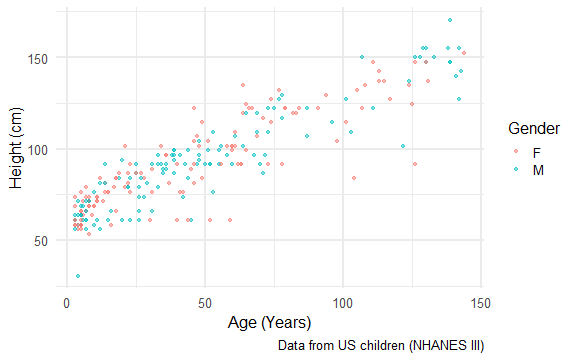
\includegraphics{chapter_files/figure-latex/unnamed-chunk-2-1.pdf}
\caption{MRP estimates from model with partial pooling}
\end{figure}

\hypertarget{sample-size-is-critical}{%
\subsection{Sample Size Is Critical}\label{sample-size-is-critical}}

MRP's performance depends heavily on the quality and size of the
researcher's survey sample. Up to now, we've been working with a random
sample of 1,000 respondents, and though the resulting estimates are
better than the raw sample means, their performance has been somewhat
underwhelming. Suppose instead we had a sample of 5,000 respondents.

\begin{Shaded}
\begin{Highlighting}[]
\NormalTok{sample\_data }\OtherTok{\textless{}{-}}\NormalTok{ ces }\SpecialCharTok{\%\textgreater{}\%} 
  \FunctionTok{slice\_sample}\NormalTok{(}\AttributeTok{n =} \DecValTok{5000}\NormalTok{)}

\CommentTok{\# fit the model}
\NormalTok{model3 }\OtherTok{\textless{}{-}} \FunctionTok{glmer}\NormalTok{(defund\_police }\SpecialCharTok{\textasciitilde{}}\NormalTok{  gender }\SpecialCharTok{+}\NormalTok{ educ }\SpecialCharTok{+}\NormalTok{ race }\SpecialCharTok{+}\NormalTok{ age }\SpecialCharTok{+}
\NormalTok{                (}\DecValTok{1} \SpecialCharTok{+}\NormalTok{ biden\_vote\_share }\SpecialCharTok{|}\NormalTok{ division), }
                 \AttributeTok{data =}\NormalTok{ sample\_data,}
                 \AttributeTok{family =} \StringTok{\textquotesingle{}binomial\textquotesingle{}}\NormalTok{)}

\CommentTok{\# construct the poststratification frame}
\NormalTok{psframe }\OtherTok{\textless{}{-}}\NormalTok{ ces }\SpecialCharTok{\%\textgreater{}\%} 
  \FunctionTok{count}\NormalTok{(abb, gender, educ, race, age, division, biden\_vote\_share)}

\CommentTok{\# make predictions}
\NormalTok{psframe}\SpecialCharTok{$}\NormalTok{predicted\_probability }\OtherTok{\textless{}{-}} \FunctionTok{predict}\NormalTok{(model3, psframe, }\AttributeTok{type =} \StringTok{\textquotesingle{}response\textquotesingle{}}\NormalTok{)}

\CommentTok{\# poststratify}
\NormalTok{poststratified\_estimates }\OtherTok{\textless{}{-}}\NormalTok{ psframe }\SpecialCharTok{\%\textgreater{}\%} 
  \FunctionTok{group\_by}\NormalTok{(abb) }\SpecialCharTok{\%\textgreater{}\%} 
  \FunctionTok{summarize}\NormalTok{(}\AttributeTok{estimate =} \FunctionTok{weighted.mean}\NormalTok{(predicted\_probability, n))}

\FunctionTok{compare\_to\_truth}\NormalTok{(poststratified\_estimates, truth)}
\end{Highlighting}
\end{Shaded}

\begin{figure}
\centering
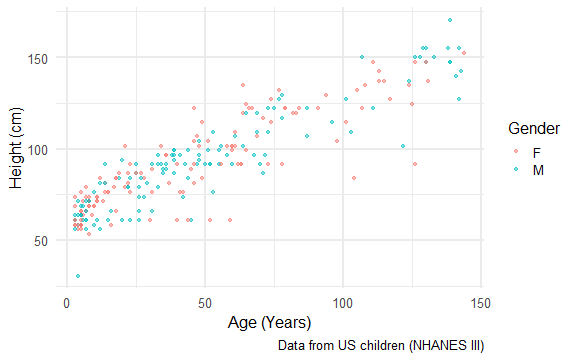
\includegraphics{chapter_files/figure-latex/unnamed-chunk-3-1.pdf}
\caption{Poststratified estimates with a survey sample of 5,000}
\end{figure}

Now MRP really shines. With more observations, the first-stage model can
better predict opinions of out-of-sample respondents, which dramatically
improves the poststratified estimates.

\hypertarget{stacked-regression-and-poststratification-srp}{%
\subsection{Stacked Regression and Poststratification
(SRP)}\label{stacked-regression-and-poststratification-srp}}

Ultimately, the accuracy of one's poststratified estimates depends on
the out-of-sample predictive performance of the first-stage model. As
we've seen above, the challenge is to thread the needle between
over-fitting and under-fitting. Several recent papers (Bisbee 2019;
Ornstein 2020; Broniecki, Leemann, and Wüest 2022) have shown that
approaches from machine learning can help to automate this process,
particularly with large survey samples.

In the code below, I'll demonstrate how an \emph{ensemble} of models --
using the same set of predictors but different methods for combining
them into predictions -- can yield superior performance to a single
multilevel regression model. In particular, I will fit a ``stacked
regression'' (Breiman 1996), which makes predictions based on a weighted
average of multiple models, where the weights are assigned by
cross-validated prediction performance (van der Laan, Polley, and
Hubbard 2007) . The literature on ensemble models is extensive, but for
good entry points I recommend Breiman (1996), Breiman (2001), and
Montgomery, Hollenbach, and Ward (2012).

\begin{Shaded}
\begin{Highlighting}[]
\CommentTok{\# construct the poststratification frame}
\NormalTok{psframe }\OtherTok{\textless{}{-}}\NormalTok{ ces }\SpecialCharTok{\%\textgreater{}\%} 
  \FunctionTok{count}\NormalTok{(abb, gender, educ, race, age, division, biden\_vote\_share)}

\CommentTok{\# fit the model (an ensemble of random forest and logistic regression)}
\FunctionTok{library}\NormalTok{(SuperLearner)}

\NormalTok{SL.library }\OtherTok{\textless{}{-}} \FunctionTok{c}\NormalTok{(}\StringTok{"SL.ranger"}\NormalTok{, }\StringTok{"SL.glm"}\NormalTok{)}

\NormalTok{X }\OtherTok{\textless{}{-}}\NormalTok{ sample\_data }\SpecialCharTok{\%\textgreater{}\%} 
  \FunctionTok{select}\NormalTok{(gender, educ, race, age, division, biden\_vote\_share)}

\NormalTok{newX }\OtherTok{\textless{}{-}}\NormalTok{ psframe }\SpecialCharTok{\%\textgreater{}\%} 
  \FunctionTok{select}\NormalTok{(gender, educ, race, age, division, biden\_vote\_share)}

\NormalTok{sl }\OtherTok{\textless{}{-}} \FunctionTok{SuperLearner}\NormalTok{(}\AttributeTok{Y =}\NormalTok{ sample\_data}\SpecialCharTok{$}\NormalTok{defund\_police,}
                       \AttributeTok{X =}\NormalTok{ X, }
                       \AttributeTok{newX =}\NormalTok{ newX, }
                       \AttributeTok{family =} \FunctionTok{binomial}\NormalTok{(),}
                       \AttributeTok{SL.library =}\NormalTok{ SL.library, }\AttributeTok{verbose =} \ConstantTok{FALSE}\NormalTok{)}
\end{Highlighting}
\end{Shaded}

\begin{verbatim}
## Error : loading required package (ranger) failed
## Error : loading required package (ranger) failed
## Error : loading required package (ranger) failed
## Error : loading required package (ranger) failed
## Error : loading required package (ranger) failed
## Error : loading required package (ranger) failed
## Error : loading required package (ranger) failed
## Error : loading required package (ranger) failed
## Error : loading required package (ranger) failed
## Error : loading required package (ranger) failed
## Error : loading required package (ranger) failed
\end{verbatim}

\begin{Shaded}
\begin{Highlighting}[]
\CommentTok{\# make predictions}
\NormalTok{psframe}\SpecialCharTok{$}\NormalTok{predicted\_probability }\OtherTok{\textless{}{-}}\NormalTok{ sl}\SpecialCharTok{$}\NormalTok{SL.predict}

\CommentTok{\# poststratify}
\NormalTok{poststratified\_estimates }\OtherTok{\textless{}{-}}\NormalTok{ psframe }\SpecialCharTok{\%\textgreater{}\%} 
  \FunctionTok{group\_by}\NormalTok{(abb) }\SpecialCharTok{\%\textgreater{}\%} 
  \FunctionTok{summarize}\NormalTok{(}\AttributeTok{estimate =} \FunctionTok{weighted.mean}\NormalTok{(predicted\_probability, n))}

\FunctionTok{compare\_to\_truth}\NormalTok{(poststratified\_estimates, truth)}
\end{Highlighting}
\end{Shaded}

\begin{figure}
\centering
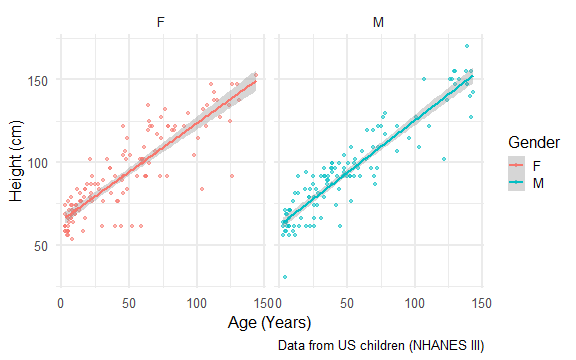
\includegraphics{chapter_files/figure-latex/unnamed-chunk-4-1.pdf}
\caption{Estimates from an ensemble first-stage model}
\end{figure}

The performance gains in Figure 7 reflect the improvement that comes
from modeling ``deep interactions'' in the predictors of public opinion
(Ghitza and Gelman 2013). If, for example, income better predicts
partisanship in some states but not in others (Gelman et al. 2007), then
a model that captures that moderating effect will produce better
poststratified estimates than one that does not. Machine learning
techniques like random forest (Breiman 2001) are especially useful for
automatically detecting and representing such deep interactions, and
stacked regression and poststratification (SRP) tends to outperform MRP
in simulations, particularly for training data with large sample size
(Ornstein 2020).

\hypertarget{synthetic-poststratification}{%
\subsection{Synthetic
Poststratification}\label{synthetic-poststratification}}

Researchers rarely have access to the entire joint distribution of
individual-level covariates. This can be limiting, since there may be
variables that one would like to include in the first-stage model, but
cannot because is not in the poststratification frame. Leemann and
Wasserfallen (2017) suggest an extension of MRP, which they
(delightfully) dub Multilevel Regression and Synthetic
Poststratification (MrsP). Lacking the full joint distribution of
covariates for poststratification, one can instead create a
\emph{synthetic} poststratification frame by assuming that additional
covariates are statistically independent of one another. So long as the
first-stage model is linear-additive, this approach yields the same
predictions as if you knew the true joint distribution!\footnote{See
  Ornstein (2020) appendix A for mathematical proof.} And even if the
first-stage model is not linear-additive, simulations suggest that the
improved performance from additional predictors tends to overcome the
error introduced in the poststratification stage.

Here are some CES covariates that we might want to include in our model
of police reform:

\begin{itemize}
\tightlist
\item
  How important is religion to the respondent?
\item
  Whether the respondent lives in an urban, rural, or suburban area
\item
  Whether the respondent or a member of the respondent's family is a
  military veteran
\item
  Whether the respondent owns or rents their home
\item
  Is the respondent the parent or guardian of a child under the age of
  18?
\end{itemize}

These variables are likely to be useful predictors of opinion about
police reform, and the first-stage model could be improved by including
them. But there is no dataset (that I know of) that would allow us to
compute a state-level joint probability distribution over every one of
them. Instead, we would typically only know the marginal distributions
of each covariate (e.g.~the percent of a state's residents that are
military households, or the percent that live in urban areas). So a
synthetic poststratification approach may prove helpful.

To create a synthetic poststratification frame, we create a set of
marginal probability distributions, and multiply them
together.\footnote{The \texttt{SRP} package contains a convenience
  function for this operation (see the
  \href{https://joeornstein.github.io/software/SRP/}{vignette} for more
  information).}

\begin{Shaded}
\begin{Highlighting}[]
\CommentTok{\# fit the model}
\NormalTok{model4 }\OtherTok{\textless{}{-}} \FunctionTok{glmer}\NormalTok{(defund\_police }\SpecialCharTok{\textasciitilde{}}\NormalTok{  gender }\SpecialCharTok{+}\NormalTok{ educ }\SpecialCharTok{+}\NormalTok{ race }\SpecialCharTok{+}\NormalTok{ age }\SpecialCharTok{+} 
\NormalTok{                  pew\_religimp }\SpecialCharTok{+}\NormalTok{ homeowner }\SpecialCharTok{+}\NormalTok{ urban }\SpecialCharTok{+} 
\NormalTok{                  parent }\SpecialCharTok{+}\NormalTok{ military\_household }\SpecialCharTok{+} 
\NormalTok{                  (}\DecValTok{1} \SpecialCharTok{+}\NormalTok{ biden\_vote\_share }\SpecialCharTok{|}\NormalTok{ division),}
                \AttributeTok{data =}\NormalTok{ sample\_data,}
                \AttributeTok{family =} \StringTok{\textquotesingle{}binomial\textquotesingle{}}\NormalTok{)}

\CommentTok{\# construct the poststratification frame}
\NormalTok{psframe }\OtherTok{\textless{}{-}}\NormalTok{ ces }\SpecialCharTok{\%\textgreater{}\%}
  \FunctionTok{count}\NormalTok{(abb, gender, educ, race, age, }
\NormalTok{        division, biden\_vote\_share) }\SpecialCharTok{\%\textgreater{}\%} 
  \CommentTok{\# convert frequencies to probabilities}
  \FunctionTok{group\_by}\NormalTok{(abb) }\SpecialCharTok{\%\textgreater{}\%} 
  \FunctionTok{mutate}\NormalTok{(}\AttributeTok{prob =}\NormalTok{ n}\SpecialCharTok{/}\FunctionTok{sum}\NormalTok{(n))}

\CommentTok{\# find the marginal distribution for each new variable}
\NormalTok{marginal\_pew\_religimp }\OtherTok{\textless{}{-}}\NormalTok{ ces }\SpecialCharTok{\%\textgreater{}\%} 
  \FunctionTok{count}\NormalTok{(abb, pew\_religimp) }\SpecialCharTok{\%\textgreater{}\%} 
  \FunctionTok{group\_by}\NormalTok{(abb) }\SpecialCharTok{\%\textgreater{}\%} 
  \FunctionTok{mutate}\NormalTok{(}\AttributeTok{marginal\_pew\_religimp =}\NormalTok{ n}\SpecialCharTok{/}\FunctionTok{sum}\NormalTok{(n))}

\NormalTok{marginal\_homeowner }\OtherTok{\textless{}{-}}\NormalTok{ ces }\SpecialCharTok{\%\textgreater{}\%} 
  \FunctionTok{count}\NormalTok{(abb, homeowner) }\SpecialCharTok{\%\textgreater{}\%} 
  \FunctionTok{group\_by}\NormalTok{(abb) }\SpecialCharTok{\%\textgreater{}\%} 
  \FunctionTok{mutate}\NormalTok{(}\AttributeTok{marginal\_homeowner =}\NormalTok{ n}\SpecialCharTok{/}\FunctionTok{sum}\NormalTok{(n))}

\NormalTok{marginal\_urban }\OtherTok{\textless{}{-}}\NormalTok{ ces }\SpecialCharTok{\%\textgreater{}\%} 
  \FunctionTok{count}\NormalTok{(abb, urban) }\SpecialCharTok{\%\textgreater{}\%} 
  \FunctionTok{group\_by}\NormalTok{(abb) }\SpecialCharTok{\%\textgreater{}\%} 
  \FunctionTok{mutate}\NormalTok{(}\AttributeTok{marginal\_urban =}\NormalTok{ n}\SpecialCharTok{/}\FunctionTok{sum}\NormalTok{(n))}

\NormalTok{marginal\_parent }\OtherTok{\textless{}{-}}\NormalTok{ ces }\SpecialCharTok{\%\textgreater{}\%} 
  \FunctionTok{count}\NormalTok{(abb, parent) }\SpecialCharTok{\%\textgreater{}\%} 
  \FunctionTok{group\_by}\NormalTok{(abb) }\SpecialCharTok{\%\textgreater{}\%} 
  \FunctionTok{mutate}\NormalTok{(}\AttributeTok{marginal\_parent =}\NormalTok{ n}\SpecialCharTok{/}\FunctionTok{sum}\NormalTok{(n))}

\NormalTok{marginal\_military\_household }\OtherTok{\textless{}{-}}\NormalTok{ ces }\SpecialCharTok{\%\textgreater{}\%} 
  \FunctionTok{count}\NormalTok{(abb, military\_household) }\SpecialCharTok{\%\textgreater{}\%} 
  \FunctionTok{group\_by}\NormalTok{(abb) }\SpecialCharTok{\%\textgreater{}\%} 
  \FunctionTok{mutate}\NormalTok{(}\AttributeTok{marginal\_military\_household =}\NormalTok{ n}\SpecialCharTok{/}\FunctionTok{sum}\NormalTok{(n))}

\CommentTok{\# merge the marginal distributions together}
\NormalTok{synthetic\_psframe }\OtherTok{\textless{}{-}}\NormalTok{ psframe }\SpecialCharTok{\%\textgreater{}\%} 
  \FunctionTok{left\_join}\NormalTok{(marginal\_pew\_religimp, }\AttributeTok{by =} \StringTok{\textquotesingle{}abb\textquotesingle{}}\NormalTok{) }\SpecialCharTok{\%\textgreater{}\%} 
  \FunctionTok{left\_join}\NormalTok{(marginal\_homeowner, }\AttributeTok{by =} \StringTok{\textquotesingle{}abb\textquotesingle{}}\NormalTok{) }\SpecialCharTok{\%\textgreater{}\%} 
  \FunctionTok{left\_join}\NormalTok{(marginal\_urban, }\AttributeTok{by =} \StringTok{\textquotesingle{}abb\textquotesingle{}}\NormalTok{) }\SpecialCharTok{\%\textgreater{}\%} 
  \FunctionTok{left\_join}\NormalTok{(marginal\_parent, }\AttributeTok{by =} \StringTok{\textquotesingle{}abb\textquotesingle{}}\NormalTok{) }\SpecialCharTok{\%\textgreater{}\%} 
  \FunctionTok{left\_join}\NormalTok{(marginal\_military\_household, }\AttributeTok{by =} \StringTok{\textquotesingle{}abb\textquotesingle{}}\NormalTok{) }\SpecialCharTok{\%\textgreater{}\%} 
  \CommentTok{\# and multiply}
  \FunctionTok{mutate}\NormalTok{(}\AttributeTok{prob =}\NormalTok{ prob }\SpecialCharTok{*}\NormalTok{ marginal\_pew\_religimp }\SpecialCharTok{*}
\NormalTok{           marginal\_homeowner }\SpecialCharTok{*}\NormalTok{ marginal\_urban }\SpecialCharTok{*}
\NormalTok{           marginal\_parent }\SpecialCharTok{*}\NormalTok{ marginal\_military\_household)}
\end{Highlighting}
\end{Shaded}

Then poststratify as normal using the synthetic poststratification
frame.

\begin{Shaded}
\begin{Highlighting}[]
\CommentTok{\# make predictions}
\NormalTok{synthetic\_psframe}\SpecialCharTok{$}\NormalTok{predicted\_probability }\OtherTok{\textless{}{-}} \FunctionTok{predict}\NormalTok{(model4, synthetic\_psframe, }
                                                   \AttributeTok{type =} \StringTok{\textquotesingle{}response\textquotesingle{}}\NormalTok{)}

\CommentTok{\# poststratify}
\NormalTok{poststratified\_estimates }\OtherTok{\textless{}{-}}\NormalTok{ synthetic\_psframe }\SpecialCharTok{\%\textgreater{}\%} 
  \FunctionTok{group\_by}\NormalTok{(abb) }\SpecialCharTok{\%\textgreater{}\%} 
  \CommentTok{\# (note that we\textquotesingle{}re weighting by prob instead of n here)}
  \FunctionTok{summarize}\NormalTok{(}\AttributeTok{estimate =} \FunctionTok{weighted.mean}\NormalTok{(predicted\_probability, prob))}

\FunctionTok{compare\_to\_truth}\NormalTok{(poststratified\_estimates, truth)}
\end{Highlighting}
\end{Shaded}

\begin{figure}
\centering
\includegraphics{chapter_files/figure-latex/unnamed-chunk-6-1.pdf}
\caption{Estimates from synthetic poststratification, including
additional covariates}
\end{figure}

\hypertarget{best-performing}{%
\subsection{Best Performing}\label{best-performing}}

As a final demonstration, suppose we had access to the entire joint
distribution over those covariates, \emph{and} our first stage model was
a Super Learner ensemble. This combination yields the best-performing
estimates yet (Figure 9).

\begin{Shaded}
\begin{Highlighting}[]
\CommentTok{\# construct the poststratification frame}
\NormalTok{psframe }\OtherTok{\textless{}{-}}\NormalTok{ ces }\SpecialCharTok{\%\textgreater{}\%} 
  \FunctionTok{count}\NormalTok{(abb, gender, race, age, educ,}
\NormalTok{        division, biden\_vote\_share,}
\NormalTok{        pew\_religimp, homeowner, urban, }
\NormalTok{        parent, military\_household)}

\CommentTok{\# fit Super Learner}
\NormalTok{SL.library }\OtherTok{\textless{}{-}} \FunctionTok{c}\NormalTok{(}\StringTok{"SL.ranger"}\NormalTok{, }\StringTok{"SL.glm"}\NormalTok{)}

\NormalTok{X }\OtherTok{\textless{}{-}}\NormalTok{ sample\_data }\SpecialCharTok{\%\textgreater{}\%} 
  \FunctionTok{select}\NormalTok{(gender, race, age, educ,}
\NormalTok{        division, biden\_vote\_share,}
\NormalTok{        pew\_religimp, homeowner, urban, }
\NormalTok{        parent, military\_household)}

\NormalTok{newX }\OtherTok{\textless{}{-}}\NormalTok{ psframe }\SpecialCharTok{\%\textgreater{}\%} 
  \FunctionTok{select}\NormalTok{(gender, race, age, educ,}
\NormalTok{        division, biden\_vote\_share,}
\NormalTok{        pew\_religimp, homeowner, urban, }
\NormalTok{        parent, military\_household)}

\NormalTok{sl }\OtherTok{\textless{}{-}} \FunctionTok{SuperLearner}\NormalTok{(}\AttributeTok{Y =}\NormalTok{ sample\_data}\SpecialCharTok{$}\NormalTok{defund\_police,}
                       \AttributeTok{X =}\NormalTok{ X, }
                       \AttributeTok{newX =}\NormalTok{ newX, }
                       \AttributeTok{family =} \FunctionTok{binomial}\NormalTok{(),}
                       \AttributeTok{SL.library =}\NormalTok{ SL.library, }
                       \AttributeTok{verbose =} \ConstantTok{FALSE}\NormalTok{)}
\end{Highlighting}
\end{Shaded}

\begin{verbatim}
## Error : loading required package (ranger) failed
## Error : loading required package (ranger) failed
## Error : loading required package (ranger) failed
## Error : loading required package (ranger) failed
## Error : loading required package (ranger) failed
## Error : loading required package (ranger) failed
## Error : loading required package (ranger) failed
## Error : loading required package (ranger) failed
## Error : loading required package (ranger) failed
## Error : loading required package (ranger) failed
## Error : loading required package (ranger) failed
\end{verbatim}

\begin{Shaded}
\begin{Highlighting}[]
\CommentTok{\# make predictions}
\NormalTok{psframe}\SpecialCharTok{$}\NormalTok{predicted\_probability }\OtherTok{\textless{}{-}}\NormalTok{ sl}\SpecialCharTok{$}\NormalTok{SL.predict}

\CommentTok{\# poststratify}
\NormalTok{poststratified\_estimates }\OtherTok{\textless{}{-}}\NormalTok{ psframe }\SpecialCharTok{\%\textgreater{}\%} 
  \FunctionTok{group\_by}\NormalTok{(abb) }\SpecialCharTok{\%\textgreater{}\%} 
  \FunctionTok{summarize}\NormalTok{(}\AttributeTok{estimate =} \FunctionTok{weighted.mean}\NormalTok{(predicted\_probability, n))}

\FunctionTok{compare\_to\_truth}\NormalTok{(poststratified\_estimates, truth)}
\end{Highlighting}
\end{Shaded}

\begin{figure}
\centering
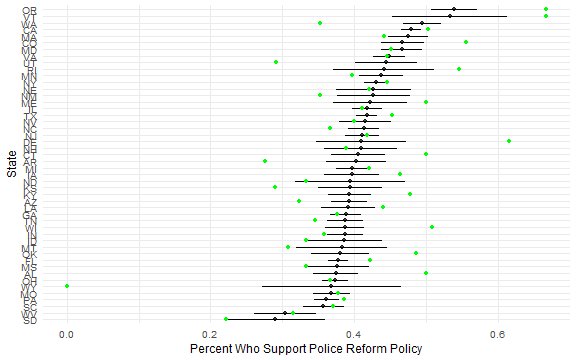
\includegraphics{chapter_files/figure-latex/unnamed-chunk-7-1.pdf}
\caption{The best performing estimates, using a large survey sample,
ensemble first stage model, and full set of predictors.}
\end{figure}

The results shown in Figure 9 reflect all the gains from a larger sample
size, ensemble modeling, and a full set of individual-level and
group-level predictors.

\hypertarget{conclusion}{%
\section{Conclusion}\label{conclusion}}

The demonstrations in this chapter suggest a number of lessons for
researchers using MRP.

First, be wary of first-stage models that are under- or over-fit to the
survey data. As we saw in Figure 3, MRP estimates with too few modeled
predictors tend to overshrink towards the grand mean.\footnote{In the
  limit, a first-stage model with zero predictors would yield identical
  poststratified estimates for each state, equal to the survey sample
  mean.} Using such estimates in a subsequent analysis would understate
the differences between regions. Conversely, models that are over-fit to
survey data (e.g.~Figure 4) will tend to exaggerate regional
differences.

Second, new techniques like synthetic poststratification and stacked
regression can help researchers manage the tradeoff between
under-fitting and over-fitting. Synthetic poststratification allows for
the inclusion of more relevant predictors, and regularized ensemble
models help ensure that the predictions are not over-fit to noisy survey
samples. The best estimates come from combining these two approaches.

Finally, recall that the most significant performance gains in our
demonstration came not from more sophisticated modeling techniques, but
from more data. As we saw in Figure 6, working with a larger survey
yielded greater marginal improvements than any tinkering around with the
first-stage modeling choices. MRP is not a panacea, and one should be
skeptical of estimates produced from small-sample surveys, regardless of
how they are operationalized.

In the code above I emphasize ``do-it-yourself'' approaches to MRP --
fitting a model, building a poststratification frame, and producing
estimates separately. But there are a number of \texttt{R} packages
available with useful functions to help ease the process. In particular,
I would encourage curious readers to explore the \texttt{autoMrP}
package (Broniecki, Leemann, and Wüest 2022), which implements the
ensemble modeling approach described above, and performs quite well in
simulations when compared to existing packages.

\hypertarget{further-suggested-readings}{%
\section{Further Suggested Readings}\label{further-suggested-readings}}

\begin{itemize}
\item
  McElreath, Richard. 2020. \emph{Statistical Rethinking: A Bayesian
  Course with Examples in R and Stan}. 2nd ed.~Boca Raton: Taylor and
  Francis, CRC Press. (particularly chapter 13).
\item
  Gelman, Andrew, Jennifer Hill, and Aki Vehtari. 2021. \emph{Regression
  and Other Stories}. Cambridge, United Kingdom: Cambridge University
  Press. (particularly chapter 17).
\end{itemize}

\hypertarget{review-questions}{%
\section{Review Questions}\label{review-questions}}

\begin{enumerate}
\def\labelenumi{\arabic{enumi}.}
\tightlist
\item
\end{enumerate}

\hypertarget{references}{%
\section*{References}\label{references}}
\addcontentsline{toc}{section}{References}

\hypertarget{refs}{}
\begin{CSLReferences}{1}{0}
\leavevmode\vadjust pre{\hypertarget{ref-achen2005}{}}%
Achen, Christopher H. 2005. {``Let's Put Garbage-Can Regressions and
Garbage-Can Probits Where They Belong.''} \emph{Conflict Management and
Peace Science} 22 (4): 327--39.
\url{https://doi.org/10.1080/07388940500339167}.

\leavevmode\vadjust pre{\hypertarget{ref-ansolabehere2015}{}}%
Ansolabehere, Stephen, Samantha Luks, and Brian F. Schaffner. 2015.
{``The Perils of Cherry Picking Low Frequency Events in Large Sample
Surveys.''} \emph{Electoral Studies} 40 (December): 409--10.
\url{https://doi.org/10.1016/j.electstud.2015.07.002}.

\leavevmode\vadjust pre{\hypertarget{ref-bisbee2019}{}}%
Bisbee, James. 2019. {``BARP: Improving Mister P Using Bayesian Additive
Regression Trees.''} \emph{American Political Science Review} 113 (4):
1060--65. \url{https://doi.org/10.1017/S0003055419000480}.

\leavevmode\vadjust pre{\hypertarget{ref-breiman1996}{}}%
Breiman, Leo. 1996. {``Stacked Regressions.''} \emph{Machine Learning}
24: 49--64. \url{https://doi.org/10.17485/ijst/2016/v9i28/98380}.

\leavevmode\vadjust pre{\hypertarget{ref-breiman2001}{}}%
---------. 2001. {``Random Forests.''} \emph{Machine Learning} 45 (1):
5--32. \url{https://doi.org/10.1023/A:1010933404324}.

\leavevmode\vadjust pre{\hypertarget{ref-broniecki2022}{}}%
Broniecki, Philipp, Lucas Leemann, and Reto Wüest. 2022. {``Improved
Multilevel Regression with Poststratification Through Machine Learning
(autoMrP).''} \emph{The Journal of Politics} 84 (1).
\url{https://doi.org/10.1086/714777}.

\leavevmode\vadjust pre{\hypertarget{ref-buttice2013}{}}%
Buttice, Matthew K., and Benjamin Highton. 2013. {``How Does Multilevel
Regression and Poststratification Perform with Conventional National
Surveys?''} \emph{Political Analysis} 21 (4): 449--67.
\url{https://doi.org/10.1093/pan/mpt017}.

\leavevmode\vadjust pre{\hypertarget{ref-gelman2018}{}}%
Gelman, Andrew. 2018. {``Regularized Prediction and Poststratification
(the Generalization of Mister p).''} \emph{Statistical Modeling, Causal
Inference, and Social Science (Blog)} May 19
(https://statmodeling.stat.columbia.edu/2018/05/19/).

\leavevmode\vadjust pre{\hypertarget{ref-gelman1997}{}}%
Gelman, Andrew, and Thomas C Little. 1997. {``Poststratification into
Many Categories Using Hierachical Logistic Regression.''} \emph{Survey
Methodology} 23 (2): 127--35.

\leavevmode\vadjust pre{\hypertarget{ref-gelman2007}{}}%
Gelman, Andrew, Boris Shor, Joseph Bafumi, and David Park. 2007. {``Rich
State, Poor State, Red State, Blue State: What's the Matter with
Connecticut?''} \emph{Quarterly Journal of Political Science} 2 (June
2006): 345--67. \url{https://doi.org/10.1561/100.00006026}.

\leavevmode\vadjust pre{\hypertarget{ref-ghitza2013}{}}%
Ghitza, Yair, and Andrew Gelman. 2013. {``Deep Interactions with MRP:
Election Turnout and Voting Patterns Among Small Electoral Subgroups.''}
\emph{American Journal of Political Science} 57 (3): 762--76.
\url{https://doi.org/10.1111/ajps.12004}.

\leavevmode\vadjust pre{\hypertarget{ref-lax2009}{}}%
Lax, Jeffrey R., and Justin H. Phillips. 2009. {``How Should We Estimate
Public Opinion in the States?''} \emph{American Journal of Political
Science} 53 (1): 107--21.
\url{https://doi.org/10.1111/j.1540-5907.2008.00360.x}.

\leavevmode\vadjust pre{\hypertarget{ref-lax2012}{}}%
---------. 2012. {``The Democratic Deficit in the States.''}
\emph{American Journal of Political Science} 56 (1): 148--66.
\url{https://doi.org/10.1111/j.1540-5907.2011}.

\leavevmode\vadjust pre{\hypertarget{ref-leemann2017}{}}%
Leemann, Lucas, and Fabio Wasserfallen. 2017. {``Extending the Use and
Prediction Precision of Subnational Public Opinion Estimation.''}
\emph{American Journal of Political Science} 61 (4): 1003--22.

\leavevmode\vadjust pre{\hypertarget{ref-montgomery2012}{}}%
Montgomery, Jacob M, Florian Hollenbach, and Michael D Ward. 2012.
{``Improving Predictions Using Ensemble Bayesian Model Averaging.''}
\emph{Political Analysis} 20 (3): 271--91.

\leavevmode\vadjust pre{\hypertarget{ref-ornstein2020}{}}%
Ornstein, Joseph T. 2020. {``Stacked Regression and
Poststratification.''} \emph{Political Analysis} 28 (2): 293--301.
\url{https://doi.org/10.1017/pan.2019.43}.

\leavevmode\vadjust pre{\hypertarget{ref-park2004}{}}%
Park, David K., Andrew Gelman, and Joseph Bafumi. 2004. {``Bayesian
Multilevel Estimation with Poststratification: State-Level Estimates
from National Polls.''} \emph{Political Analysis} 12 (4): 375--85.
\url{https://doi.org/10.1093/pan/mph024}.

\leavevmode\vadjust pre{\hypertarget{ref-schaffner2021}{}}%
Schaffner, Brian, Stephen Ansolabehere, and Sam Luks. 2021.
{``Cooperative Election Study Common Content, 2020.''} Edited by YouGov
and Add your team name(s) here.
\url{https://doi.org/10.7910/DVN/E9N6PH}.

\leavevmode\vadjust pre{\hypertarget{ref-tausanovitch2014}{}}%
Tausanovitch, Chris, and Christopher Warshaw. 2014. {``Representation in
Municipal Government.''} \emph{The American Political Science Review}
108 (03): 605--41. \url{https://doi.org/10.1017/S0003055414000318}.

\leavevmode\vadjust pre{\hypertarget{ref-vanderlaan2007}{}}%
van der Laan, Mark J., Eric. C. Polley, and Alan E. Hubbard. 2007.
{``Super Learner.''} \emph{Statistical Applications in Genetics and
Molecular Biology} 6 (1).

\leavevmode\vadjust pre{\hypertarget{ref-wang2015}{}}%
Wang, Wei, David Rothschild, Sharad Goel, and Andrew Gelman. 2015.
{``Forecasting Elections with Non-Representative Polls.''}
\emph{International Journal of Forecasting} 31 (3): 980--91.
\url{https://doi.org/10.1016/j.ijforecast.2014.06.001}.

\end{CSLReferences}

\end{document}
